\documentclass[11pt]{article}

\usepackage{mathtools}
\usepackage{amssymb}
\usepackage{amsmath}
\usepackage{amsthm}
\usepackage{hyperref}
\usepackage{microtype}
\usepackage{graphicx}
\graphicspath{ {./img/} }

\setlength{\parindent}{0cm}
\let\emptyset\varnothing

\title{\textbf{CSCI/MATH 2113 Discrete Structures} \\ 5.5 The Pigeonhole Principle}
\author{Alyssa Motas}

\begin{document}

    \maketitle

    \pagebreak

    \tableofcontents

    \pagebreak

    \section{The Pigeonhole Principle}

    \subsection{Definition}

    If $m$ pigeons occupy $n$ pigeonholes and $m > n$ then at least one pigeonhole has two or more pigeons in it.

    \subsection{Example}

    If there are 5 points in a \(2 \times 2\) square in the real plane, then two of these points are no more than \(\sqrt{2}\) away from each other. 

    \begin{center}
        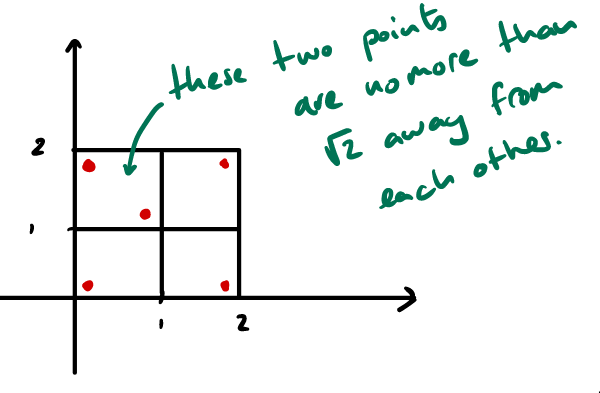
\includegraphics[scale=0.5]{ex.png}
    \end{center}


\end{document}